\chapter{Nuclear Reactions}\label{ch:iv}

\section{Introduction} 

Most observed stars, including the Sun, are powered by thermonuclear fusion. This term denotes nuclear reactions induced by the thermal motion of the ions, wherby lighter nuclei comnine to form a heavier one.
\par If the combined mass of the interacting nuclei is larger than the mass of the produced nucleus, the mass difference is converted into energy according to the famous (to the point of being obnoxious) Einstein's relation.
\par The mass difference between the interacting protons and the product of their interaction stems for the properties of the nuclear binding energy $E_{B}$, which is the energy required to separate nucleons against their mutual attraction due to nuclear forces, and is essentially a measure of the stability of the nucleus.
\begin{figure}[h!]
    \centering 
    \includegraphics[width=0.7\textwidth]{img/bindingenergy.svg.png}
    \caption{Binding energy per nucleon for a selection of nuclides. The nuclide with the highest value, $^{62}\text{Ni}$, is noted.}
    \label{fgr:bindingenergy}
\end{figure}
\par The binding energy per nucleon, shown in Fig.\ref{fgr:bindingenergy} is a most interesting quantitiy; its value increases with $A$ first steeply, then more gently, until it reaches a maximum of $8.79\,\text{MeV}$ around $A=56$, which corresponds to $^{56}\text{Fe}$, and then drops slowly for heavier nucleons.
\par Most people claim, for reasons we'll soon find out, that Iron nuclei are the most stable ones, while it's false. It's actually $^{62}\text{Ni}$ nuclei that claim this figurative top position.
\par Elements up to Iron (read: Nichel) will therefore produce energy by thermonuclear fusion, whereas for higher values of $A$ it is the splitting of heavier nuclei into ligther ones (\emph{nuclear fission}) that does the deed.
\par We'll now focus on the determination of the nuclear energy generation coefficient.
\section{Energy Production Rate}
Consider a reaction of the type
\begin{equation*}
    \text{A}+\text{b}\to \text{C}+\text{d}
\end{equation*}
in which the target nucleus A interacts with the particle b and forms nucleus C plus particle d. Three (or more) body interactions have a much smaller probability of happening and can therefore be neglected to a first approximation\footnote{We're going to have to consider at least one of those if we want to produce heavier elements.}.
\par We define a cross section $\sigma$ as the number of reactions per target nucleus per unit time, divided by the number of incident particles per unit area per unit time. By denoting with $v$ the relative velocity of species A and b, the number of reactions $r$ is given by $r = v\sigma(v)N_{A}N_{b}$, but since particles in stellar gas have a non-negligible velocity distribution, we'll have to integrate over the whole allowed range of velocities
\begin{equation}
    r = N_{A}N_{b}\int_{0}^{\infty}v\sigma(v)f(v)\,\text{d}v = \frac{N_{A}N_{b}}{1+\delta_{Ab}}\langle \sigma v \rangle
    \label{eq:reactionrate}
\end{equation}
where $\delta_{Ab}$ is a Kronecker delta. By recalling that the mass fraction of a generic element $k$ is given by 
\begin{equation*}
    X_{k} = \frac{N_{k}m_{\text{H}A_{k}}}{\rho}
\end{equation*}
we get the following expression for the reaction rate per unit mass
\begin{equation}
    R_{Ab} = \rho \frac{X_{A}X_{b}}{m_{\text{H}}^{2}A_{A}A_{b}} \frac{\langle \sigma v \rangle_{Ab}}{1+\delta_{Ab}}
\end{equation}
and the nuclear energy generation coefficient can be therefore written as 
\begin{equation}
    \epsilon_{N} = R_{Ab}Q_{Ab}
\end{equation}
with $Q_{Ab}$ being the amount of energy released by a single reaction. The value of $Q_{Ab}$ can be determined from the difference between the sum of the masses of the interacting particles and the sum of the masses of the products
\begin{equation}
    Q = \sum_{r} m_{r}(c^{2}) - \sum_{p}m_{p}(c^{2})
    \label{eq:qvalue}
\end{equation}
Often nuclear masses are expressed in atomic mass units, and \cite{2005essp.book.....S} points out that is worth recalling that $931.494\,\text{MeV}$ is the amount of energy associated with one mass unit ($1.6605\cdot 10^{-24}\,\text{g}$). Moreover, if a positron is produced by the nuclear reaction, it is customary to add to $Q_{Ab}$ its annihilation energy, whereas, in the case neutrinos are produced, their energy has to be subtracted from the total energy production budget.
\par In order to determine $\epsilon_{N}$ we still have to discuss how $\langle \sigma v \rangle$ can be determined. Matter involved in nuclear reactions is well approximated by a fully ionize perfect gas, and the particle velocities and kinetic energies follow the well-known Maxwellian distribution. 
\par If the individual particles have a maxwell velocity distribution, it is possible to show that their relative velocities $v$ will also follow the same distribution. Since the corresponding kinetic energy is $E = \mu v^{2}/2$, where $\mu$ is the reduced mass of the interacting particles, the expression for $\langle \sigma v \rangle$ thus becomes
\begin{equation*}
    \langle \sigma v \rangle = \left(\frac{8}{\pi \mu}\right)^{1/2}\frac{1}{(kT)^{3/2}}\int_{0}^{\infty}\sigma(E)E e^{-E/kT}\,\text{d}E
\end{equation*}
but in order to complete the calculation we need further information about the dependence of $\sigma(E)$ on the energy $E$. This, of course, can be done by studying the process of thermonuclear fusion in more detail.
\par Whenever a pair of particles A and b interacts (that is, whenerver they come close enough that the attractive nuclear force tends to fuse them together) a compound nucleus C' is formed, with atomic and mass number that is the sum of the respective numbers of its "progenitors". 
\par Clearly, the nucleus C' has no memory of how it was formed. 
\par This compound nucleus is in a particular excited state for a given time $\tau$, after which it'll break up in many possible ways, producing, among the various possibilities, the particles C and d.
\par The probability that our generic reaction $\text{A}+\text{b}\to \text{C}+\text{d}$ is really happening, depends on the product of the probability that the interacting particles come close enough to experience the effect of the attractive nuclear force, and the probability that this interaction produces the particles C and d.
\par In order to obtain the fusion of charged particles, they have to be able to get close enough that the short range forces dominate over the long range repulsive Coulombian forces. Nuclear attraction dominates for distances that are of the order of the nuclear size, so $\sim 10^{-13}\,\text{cm}$. For larger distances, the repulsive electrostatic potential prevails
\begin{equation*}
    V_{\text{Coulomb}} = \frac{Z_{A}Z_{b}e^{2}}{r}
\end{equation*}
where $Z_{A}$, $Z_{b}$ are the electric charges of A and b. Clearly, the electrostatic potential barrier can be overcome only if particles have a kinetic energy of the same order $kT \sim V_{\text{Coulomb}}$, which, for all but few cases, it's physically impossible.
\par Then how come nuclear reactions are indeed happening in the cores of stars?
\par As was investigated by G. Gamow \cite{1928Nature}, there is a small but quite finite probability of 'tunnelling' through the Coulombian potential barrier, even for particles of energy lower than $ V_{\text{Coulomb}}$. It can be shown that the probability of tunnelling, in terms of the energy $E$ of the relative motion of the colliding particles is
\begin{equation}
    P_{G} = p_{0}e^{-b/E^{1/2}} \quad b = \left(\frac{\mu}{2}\right)^{1/2}\left(\frac{2\pi Z_{A}Z_{b}e^{2}}{\hbar}\right)
    \label{eq:gamowprob}
\end{equation}
Through this miracle, nuclear fusion can happen at temperatures much lower than predicted by classical physics.
\par At a given $E$ the probability decreases for increasing $Z_{A}$, $Z_{b}$ (the potential barrier gets higher), and progressively higher temperatures are needed for nuclear 'burnings' involving heavier nuclei.
\begin{figure}[h!]
    \centering
    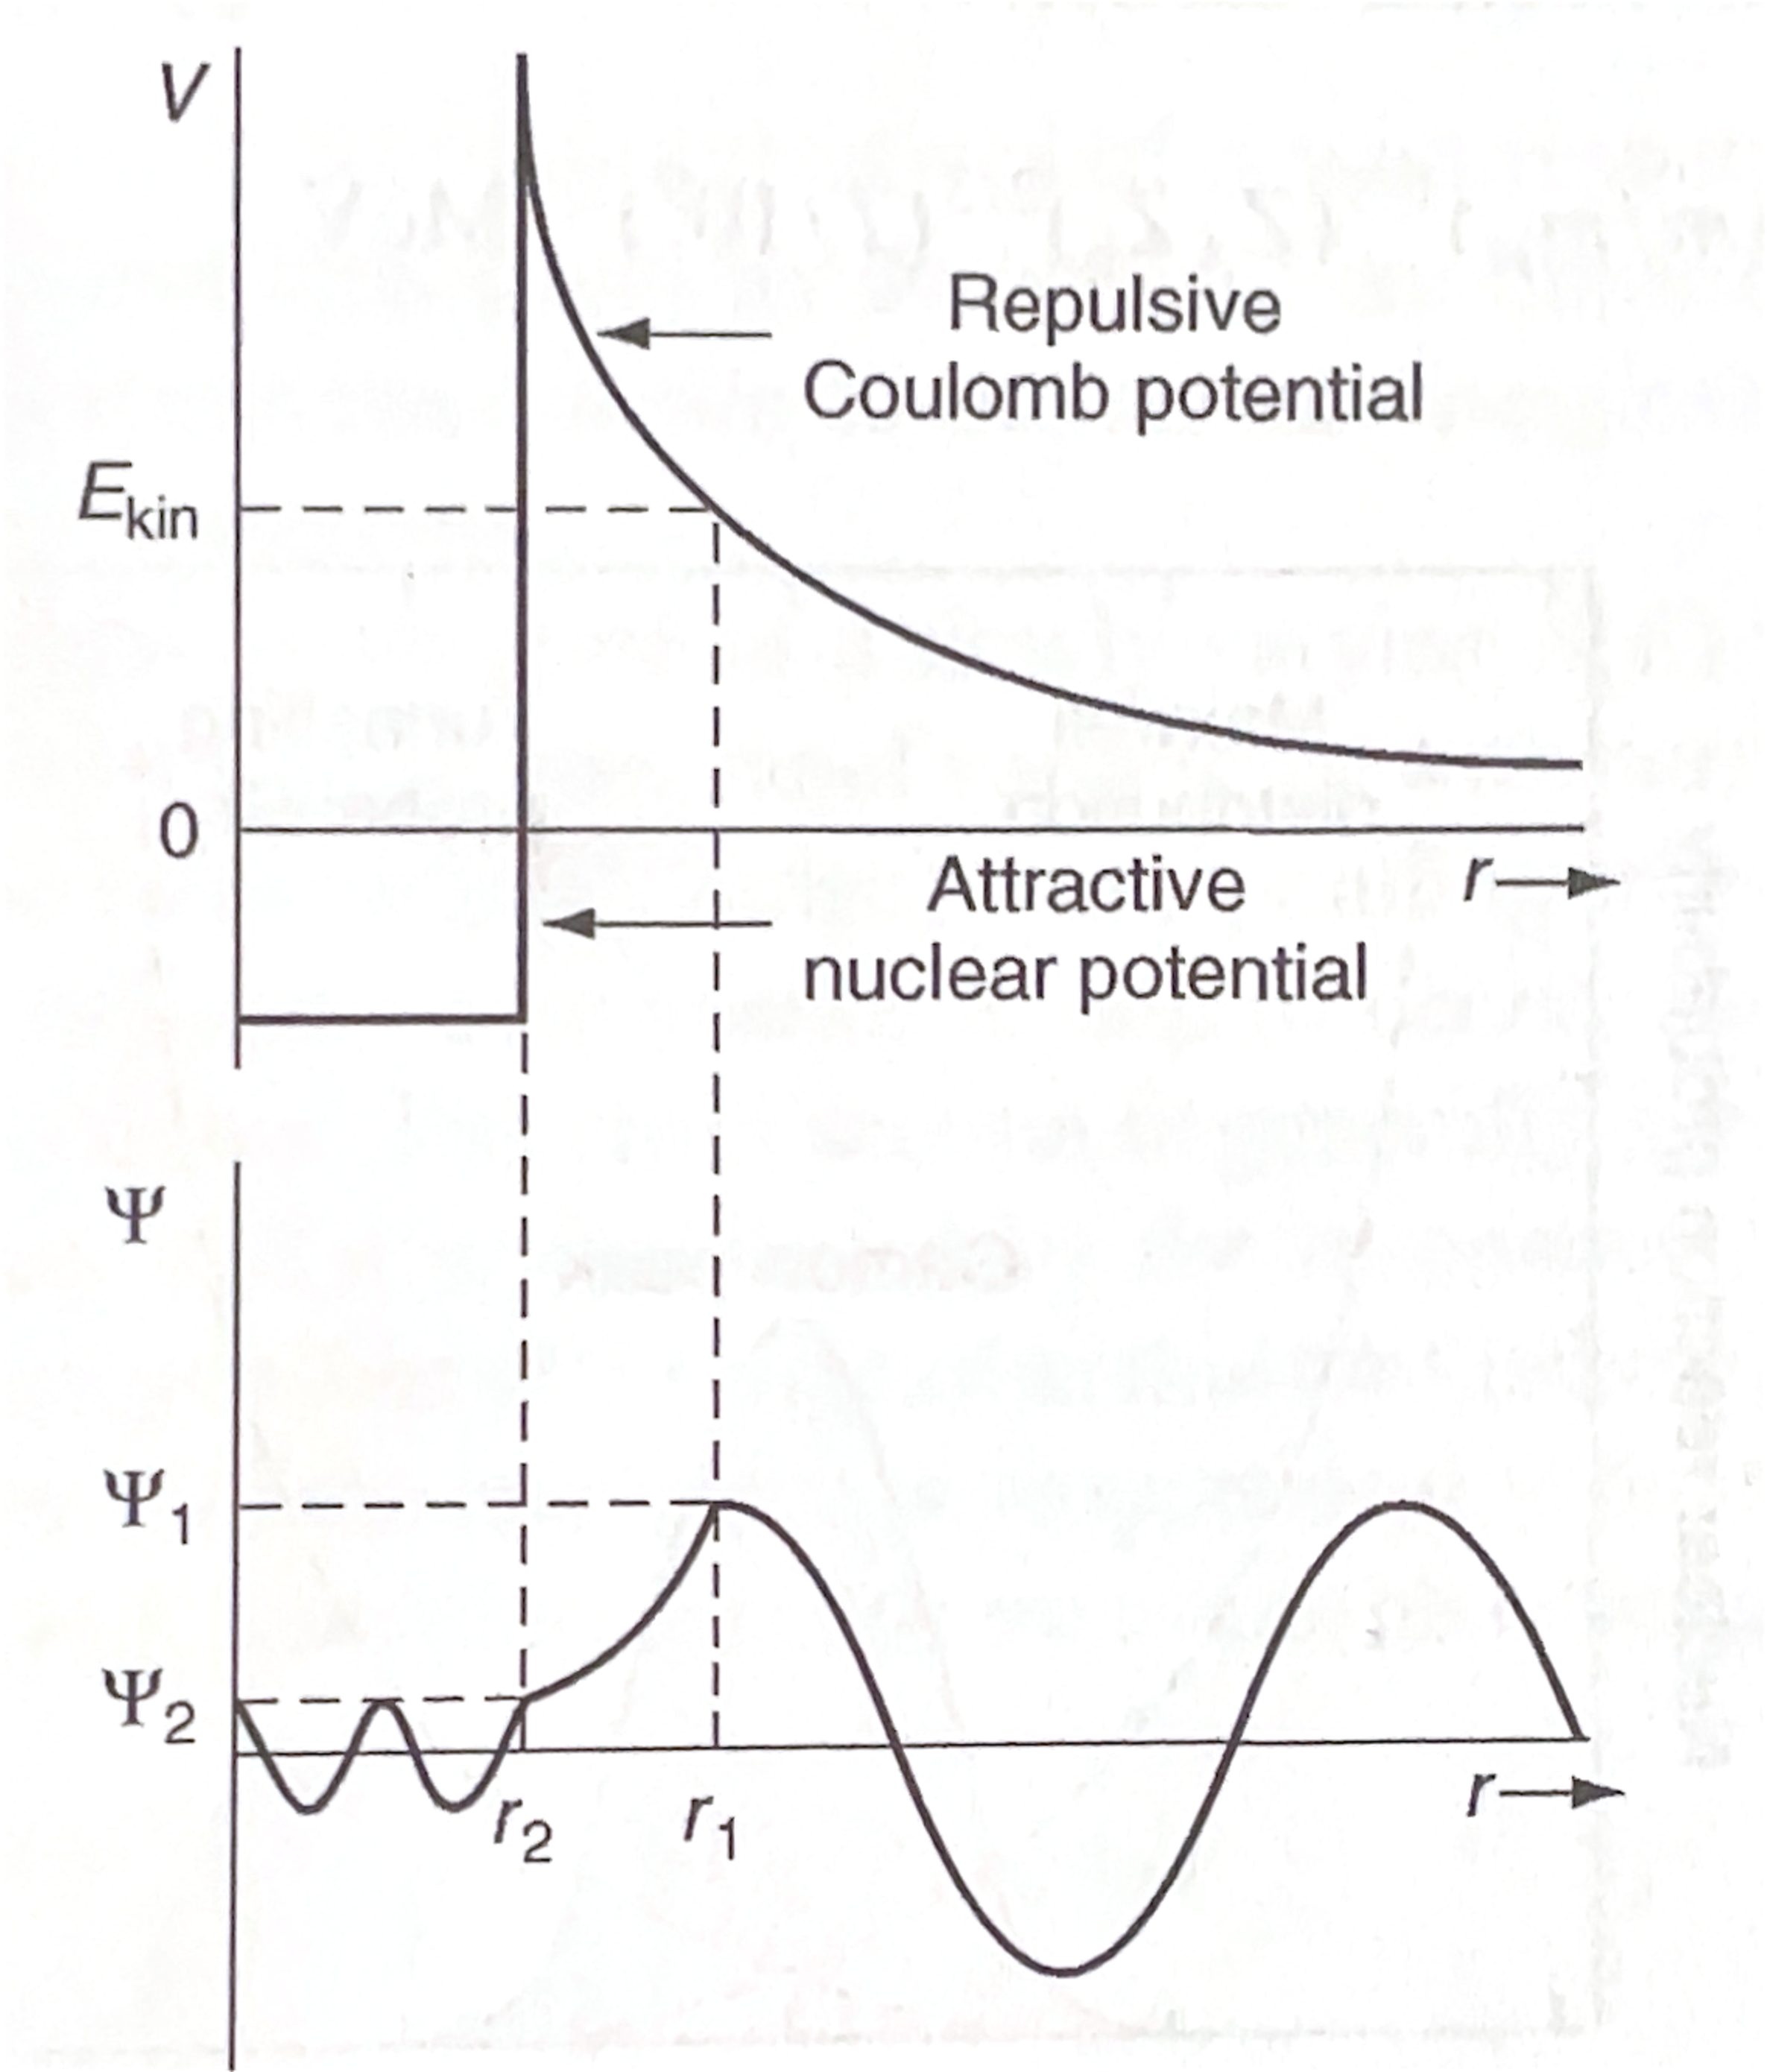
\includegraphics[width=0.4\textwidth]{img/Repulsive.pdf}
    \caption{Illustration of the potential seen by a particle b when approaching a particle A with a kinetic energy $E_{\text{kin}}$ and the corresponding wavefunction $\Psi$. Credits: \cite{2005essp.book.....S}.}
    \label{fgr:tunnelling}
\end{figure}
\par In astrophysics it is customary to define the quantity 
\begin{equation}
    S(E) = \sigma(E) E e^{+b/E^{1/2}}
    \label{eq:astrophysicalfactor}
\end{equation}
called \emph{astrophysical factor}, that is mainly sensitive to the nuclear contribution to the cross section. We may now rewrite the equation for $\langle \sigma v \rangle$ by including $S(E)$
\begin{equation}
    \langle \sigma v \rangle = \left(\frac{8}{\mu\pi}\right)^{1/2}\frac{1}{(kT)^{3/2}}\int_{0}^{\infty}S(E)\exp\left(-\frac{E}{kT}-\frac{b}{\sqrt{E}}\right)\,\text{d}E
    \label{eq:averagenuclearcs}
\end{equation}
In many cases of astrophysical relevance, the so-called non-resonant reactions, $S(E)$ is a slowly varying function of $E$ in the range of interest. Note how in (\ref{eq:averagenuclearcs}) the first term of the exponential represents the high energy wing of the Maxwellian distribution, while the second one represents the energy dependence of the tunnelling probability. Sometimes a scale energy $E_{\text{Gamow}}$ is defined, so that $b^{2} = E_{\text{Gamow}}$.
\begin{figure}[h!]
    \centering
    \includegraphics[width=0.6\textwidth]{img/Gamow_peak.png}
    \caption{Illustration of the location and shape of the Gamow peak (not to scale) as compared with $e^{-E/kT}$ and $e^{-b/\sqrt{E}}$.}
    \label{fgr:gamowpeak}
\end{figure}
\par Their product, shown in Fig.\ref{fgr:gamowpeak}, produces a strongly peaked curve, with a maximum at the so-called \emph{Gamow peak}, which also represents the most efficience energy for the nuclear reaction to occur.
\par The energy $E_{0}$ of the peak is 
\begin{equation}
    E_{0} = \left(\frac{bkT}{2}\right)^{2/3} \approx 0.122\left(\frac{\mu}{m_{\text{H}}}\right)^{1/3}(Z_{A}Z_{b})^{2/3}\left(\frac{T}{10^{9}\,\text{K}}\right)^{2/3}\,\text{MeV}
    \label{eq:gamowpeak}
\end{equation}
and the FWHM $\Delta E_{0}$ is given by
\begin{equation}
    \Delta E_{0} \sim 0.237 \left(\frac{Z_{A}^{2}Z_{b}^{2}\mu}{m_{\text{H}}}\right)^{1/6}\left(\frac{T}{10^{9}\,\text{K}}\right)^{5/6}\,\text{MeV}
    \label{eq:gamowfwhm}
\end{equation}
It is in the Gamow peak energy range that S(E) needs to be known in order to derive the reaction rate. Unfortunately, this energy range is at least a factor of 10 lower than the energies at which stellar reactions can be produced in laboratories; therefore, all we're able to do is extrapolate the measured $S(E)$ values to much lower energies if an empirical determination of $S(E)$ is sought.
\par As mentioned somewhere in the above, the astrophysical factor is often a slowly varying function of energy, and (\ref{eq:averagenuclearcs}) is usually solved considering a second-order Taylor expansion for $S$ and $e^{-b/\sqrt{E}}$ around $E_{0}$. If we approximate the exponential term as a Gaussian function\footnote{It is actually not a bad approximation, but the curve is slightly skewed, so we'll have to make some corrections afterwards.} 
\begin{equation*}
    I_{\text{max}} \approx \exp\left(-\frac{E}{kT}-\sqrt{\frac{E_{G}}{E}}\right) \implies I_{\text{max}} \approx I(E_{0})
\end{equation*}
meaning 
\begin{equation*}
    I_{\text{max}} = \exp\left(-\frac{3E_{0}}{kT}\right) = \exp(-\tau)
\end{equation*}
This way we can write 
\begin{equation*}
    I_{\text{max}} = e^{-\tau}\exp\left[-\left(\frac{E-E_{0}}{\Delta/2}\right)^{2}\right] \quad \Delta = \text{FWHM}
\end{equation*}
Once plugged in (\ref{eq:averagenuclearcs}), this provides 
\begin{equation}
    \langle \sigma(v)v \rangle = \sqrt{\frac{2}{\mu}}\frac{\Delta}{(kT)^{3/2}}S_{\text{eff}}\,e^{-3E_{0}/kT}
    \label{eq:approximatenuclearrt}
\end{equation}
with 
\begin{equation}
    \frac{S_{\text{eff}}}{S(E_{0})} = 1+\frac{5kT}{36E_{0}}+\frac{S'(E_{0})}{S(E_{0})}\left(E_{0}+\frac{35}{36}kT\right)+\frac{1}{2}\frac{S''(E_{0})}{S(E_{0})}\left(E_{0}^{2}+\frac{89}{36}kTE_{0}\right)
    \label{eq:effectiveastrofactor}
\end{equation}
The values for the astrophysical factor and its derivaties are obtained either from laboratory measurements (with the aforementioned limitations) or from theoretical quantum mechanical computations.
\par Let's see how can we deduce the (approximate) temperature dependence. Say $T_{0}$ a reference temperature, which may be the temperature for which the burning of a particular element is possible.
\par We've shown that in general, the energy at Gamow's peak is dependent on the temperature 
\begin{equation*}
    E_{0} = \left(\frac{bkT}{2}\right)^{2/3} \quad b = \frac{(2\mu)^{1/2}\pi e^{2}Z_{A}Z_{b}}{\hbar}
\end{equation*}
Let us expand (\ref{eq:averagenuclearcs}) around our reference temperature in the way presented below 
\begin{equation*}
    \langle \sigma v \rangle_{T} \approx  \langle \sigma v \rangle_{T_{0}}\left(\frac{T}{T_{0}}\right)^{\nu}
\end{equation*} 
Taking the logarithms of both memebers
\begin{equation*}
    \ln( \langle \sigma v \rangle_{T}) \approx \ln( \langle \sigma v \rangle_{T_{0}})+\nu\ln\left(\frac{T}{T_{0}}\right)
\end{equation*}
hence 
\begin{equation*}
    \nu \approx \frac{ \ln( \langle \sigma v \rangle_{T}) - \ln( \langle \sigma v \rangle_{T_{0}})}{\ln T -\ln T_{0}} = \der{\ln\langle \sigma v \rangle}{\ln T}\Big|_{T=T_{0}}
\end{equation*}
Let us express this in terms of the variable $\tau = 3E_{0}/kT$ we've used earlier when expanding the exponential term in (\ref{eq:averagenuclearcs}).
\par You can show that 
\begin{equation*}
    \tau \propto T^{-1/3}\implies T\propto \tau^{-3} \implies \ln T = C-3\ln\tau
\end{equation*}
while for $\langle \sigma v \rangle_{T}$ we use (\ref{eq:approximatenuclearrt}). Let's explicit the various dependencies
\begin{equation*}
    \langle \sigma v \rangle_{T} \propto \frac{\Delta}{T^{3/2}}e^{-\tau} \quad \Delta \propto T^{5/6}
\end{equation*}
which, after putting all together, implies 
\begin{equation*}
    \langle \sigma v \rangle_{T} \propto T^{-2/3}e^{-\tau} \propto \tau^{2}e^{-\tau} \implies \ln\langle \sigma v \rangle_{T} \propto D +2\ln\tau -\tau
\end{equation*}
Now we can finally plug everything in the definition of $\nu$. Calculating
\begin{equation*}
    \text{d}\ln\langle \sigma v \rangle_{T} = \text{d}\tau\left(\frac{2}{\tau}-1\right) \quad \text{d}\ln T = -\frac{3}{\tau}\text{d}\tau
\end{equation*}
\begin{equation*}
    \nu = \der{\ln\langle \sigma v \rangle}{\ln T}\Big|_{T=T_{0}} = -\frac{2}{3}+\frac{\tau}{3}
\end{equation*}
meaning that 
\begin{equation}
    \boxed{
    \langle \sigma v \rangle \propto T^{-\frac{1}{3}(\tau_{0}-2)}
    }
    \label{eq:nrtemperaturedep}
\end{equation}
For example, consider a reaction from the $\text{ppI}$ chain
\begin{equation*}
    p+p \to D + e^{+}+\bar{\nu}_{e} \implies \langle \sigma v \rangle\propto T^{4}
\end{equation*}
\subsection{Resonant Reactions}
So far we've been focusing on reactions for which the astrophysical factor (\ref{eq:astrophysicalfactor}) was slowly varying with energy, the so-called \emph{non-resonant reactions}. We've mentioned before that given two reactants, multiple products are possible, depending on the nature of the interaction (elastic, anelastic, etc).
\begin{align*}
    \text{A}+\text{b} \to \text{C}^{*} &\to \text{A}+\text{b} \; (\text{elastic scattering})\\
                  &\to \text{A}+\text{b}^{*}\; (\text{anelastic scattering})\\
                  &\to \text{D}+\text{e}\\
                  &\to \text{C}+\gamma\; (\text{radiative capture})\\
\end{align*}
Note that if the energy of the center of mass added to the Q-value of the specific reaction is "close enough" to one of the energetic level of the compound nucleus C$^{*}$, then the reaction is \emph{resonant}. We'll consider only \emph{narrow} resonant reactions, for which the width of the resonance is much smaller than the resonant energy 
\begin{equation}
    \Gamma \ll E_{R}
    \label{eq:narrowresonance}
\end{equation}
It should come as no surprise that, around resonance, the interaction cross section becomes extremely larger, and it's no more the one we've found in (\ref{eq:averagenuclearcs}), but it's rather the one found by Breit and Wigner
\begin{equation}
    \sigma_{BW}(E) = \frac{\lambda^{2}}{4\pi}\frac{\omega\Gamma_{1}\Gamma_{2}(1+\delta_{Ab})}{(E-E_{R})^{2}+\left(\frac{\Gamma}{2}\right)^{2}}
    \label{eq:breitwignercs}
\end{equation}
where $\lambda$ is the De-Broglie wavelength
\begin{equation}
    \lambda = \frac{h}{\sqrt{2\mu E}}
    \label{eq:debrogliewavelength}
\end{equation}
and $\Gamma_{1}$ is the probability amplitude of forming the compound nucleus, which is also equal to its decay probability; $\Gamma_{2}$ is the probability amplitude of decaying in the products of the reaction (say D, e), while $\Gamma$ is the width of the excited level responsible of the resonance. Note that $\Gamma$ is proportional to the total lifetime $\tau$ of the excited state according to 
\begin{equation}
    \Gamma = \frac{h}{2\pi\tau}
    \label{eq:branchingfraction}
\end{equation}
and $\Gamma_{1}$, $\Gamma_{2}$ have a similar definition, but considering the lifetime for the decay of the compound nucleus into the original interacting particles A+b, and into the products D+e, respectively. In teh case of heavy compound nuclei many resonances are present in the range of stellar energies.
\par On the other hand, the factor $\omega$ is related to the spin of the reactants and to the (total) angular momentum of the compound nucleus
\begin{equation*}
    \omega = \frac{2J+1}{(2J_{A}+1)(2J_{b}+1)}
\end{equation*}
At this point we can write anew the reaction rate (\ref{eq:reactionrate}), but with a few caveats. First of all, now we're in the presence of a narrow resonance, meaning that if the Gamow peak $E_{0}$ is far from resonance $E_{R}$, we won't be able to observe the resonance.
\par On the other hand, if $E_{R}\sim E_{0}$, the resonance overrides all the other possible decay products, and thus we have to use (\ref{eq:breitwignercs}) rather than the tunnelling probability.
\par We still have to average over the velocity distribution
\begin{equation}
    \langle \sigma v \rangle = \left(\frac{8}{\pi\mu}\right)^{1/2}\frac{1}{(kT)^{3/2}}\int_{0}^{\infty}\sigma_{BW}(E)Ee^{-E/kT}\,\text{d}E
    \label{eq:resonanrreactionrate}
\end{equation}
But since the resonance is narrow around $E_{R}$ and, for extension, around $E_{0}$, we can bring the Maxwellian contribution out of the integral, evaluating them in $E_{R}$
\begin{equation*}
    \langle \sigma v \rangle = \left(\frac{8}{\pi\mu}\right)^{1/2}\frac{1}{(kT)^{3/2}}E_{R}e^{-E_{R}/kT}\int_{0}^{\infty}\sigma_{BW}(E)\,\text{d}E
\end{equation*}
\par This integral can be calculated, thus finding
\begin{equation}
    \langle \sigma v \rangle = \left(\frac{2\pi}{\mu kT}\right)^{3/2}\hbar^{2}\omega\gamma e^{-E_{R}/kT}
        \label{eq:narrowresonanrreactionrate}
\end{equation}
where $\gamma = \Gamma_{1}\Gamma_{2}/\Gamma$. Unlike narrow resonances, \emph{broad resonances} are more troublesome, since they have broad tails that can influence the interaction cross section even when the reaction is well out of resonance conditions.
\subsection{Electronic Shielding}
It is important to notice that in our previous discussion and the cross sections provided in the literature refer to reactions \emph{happening in vacuum}. Instead, as I'm sure the sharpest among my four readers had been itching to point out for a while, ions in stellar interiors are surrounded by a sea of free electrons that tend to cluster near the nuclei and reduce their Coulomb potential.
\par Therefore an approaching particle will feel a Coulombian potential different from the case of an isolated positive charge. This shielding effect of the electrons increases the reaction rate $\langle \sigma v \rangle$ by a so-called \emph{screening factor} $f$ that will necessarily be a function of the matter density.
\par Consider the upper cartoon of Fig.\ref{fgr:tunnelling}, and assume that the impinging particle on our target nucleus has an energy much lower than the Coulombian potential. The poor thing would not be able to interact effectively with the target nucleus and will "stop" at a distance known as \emph{classical turning point}, which is easily computed 
\begin{equation}
    r_{TP} = \frac{Z_{A}Z_{b}e^{2}}{E_{b}}
    \label{eq:classicalturningpointradius}
\end{equation}
In reality, however, the target nucleus has some electrons, that will be located at a certain distance from the nucleus. Within the electronic cloud, the Coulombian potential vanishes.
\par Then, if our impinging projectile had an energy such that $r_{TP}>r_{A}$, where $r_{A}$ is the atomic radius, the resulting effect would be incredible since, because of the electronic shielding, the effective electrostatic potential would be identically zero.
\par Let us define an energy 
\begin{equation*}
    U_{e} = \frac{Z_{A}Z_{b}e^{2}}{r_{A}}
\end{equation*}
so that if $E_{b}>U_{e}$, the projectile can break into the electronic cloud. This is indeed what happens, since $U_{e}$ is rather small ($\sim 0.03\,\text{keV}$). If that is the case, then necessarily $r_{TP}<r_{A}$.
\par So how does the electrostatic potential changes? We can imagine the cloud as a symmetric source of potential around $Z_{A}$, so that
\begin{equation*}
    \Phi_{A} = -\frac{Z_{A}e}{r_{A}}
\end{equation*}
Therefore the total potential within the cloud decreases a bit
\begin{equation*}
    \Phi_{\text{tot}} = \frac{Z_{A}e}{r}-\frac{Z_{A}e}{r_{A}}
\end{equation*}
but we're interested in evaluating it at distances comparable to the range of nuclear forces, where our nuclear fusion interactions can take place.
\par This has the effect of lowering the Coulombian barrier
\begin{equation*}
    V_{\text{eff}} = \frac{Z_{A}Z_{b}e^{2}}{r_{N}}-\frac{Z_{A}Z_{b}e^{2}}{r_{A}}
\end{equation*}
The correction we've introduced is rather small, since $r_{N}/r_{A}\sim 10^{-5}$. In a sense, we could consider this effect as an increased energy of the impinging projectile $E_{b}\to E_{b}+U_{e}$. This clearly induces a slight increasing of the reaction rate by a factor $f$.
\par The shielding factor $f$ is defined as 
\begin{equation}
    f = \frac{\sigma(E_{b}+U_{e})}{\sigma(E_{b})}
    \label{eq:shieldingfactor}
\end{equation}
Albeit small, this effect is not at all negligible. From the definition (\ref{eq:shieldingfactor}) we can substitute the expressions for the cross sections (I'm dropping the b-subscript)
\begin{equation*}
    \frac{\sigma(E+U_{e})}{\sigma(E)} = \frac{E}{E+U_{e}}\frac{S(E+U_{e})}{S(e)}\exp\left(-\frac{2\pi Z_{A}Z_{b}e^{2}\sqrt{\mu}}{\hbar\sqrt{2(E+U_{e})}}+\frac{2\pi Z_{A}Z_{b}e^{2}\sqrt{\mu}}{\hbar\sqrt{2E}}\right)
\end{equation*}
which, since $U_{e} \ll E$, we can Taylor-expand. First of all we can notice that the first two ratios are, at linear order, of order unity. Then, expanding the square root, we obtain
\begin{equation*}
    f \approx \exp\left(\frac{\pi Z_{A}Z_{b}e^{2}\sqrt{\mu}}{\hbar\sqrt{2E}}\frac{U_{e}}{E}\right)
\end{equation*}
which becomes more and more relevant for lower energies of the center of mass, which are those of astrophysical relevance, since the astrophysical factor starts to climb up back again.
\par To the reaction rates we've been calculating so far we have to add a correction to address the effect of electronic shielding in the stellar plasma. The idea is that, although the stellar plasma is globally neutral, whenever a impinging projectile comes close to an ionized nucleus, the two charged nuclei start repelling each other, whilst electrons tend to be attracted.
\par If that's the case, then we can imagine our stellar plasma as made of a myriad of charged nuclei that are getting "shielded" by electronic clouds at a certain distance from them, so that when a nucleus interact with another nucleus, the electronic cloud, which is just an electron over-density, trails behind it.
\par Say that $n_{i}$ is the numeric density of the ions
\begin{equation*}
    n_{i} \approx \frac{\rho}{\mu_{i}m_{\text{H}}} \approx \frac{1}{\frac{4\pi}{3}a^{3}}
\end{equation*}
with $a$ the average distance between ions. We can invert the latter expression
\begin{equation*}
    a \sim \frac{1}{n_{i}^{1/3}} \sim \left(\frac{\mu_{i}n_{\text{H}}}{\rho}\right)^{1/3}
\end{equation*}
In the inner regions of the stellar plasma, the density is quite large, meaning that the distance between two ions gets smaller.
\par We can define \emph{strong shielding} the condition for which 
\begin{equation}
    \frac{Z_{1}Z_{2}e^{2}}{akT} \gg 1
    \label{eq:strongshielding}
\end{equation}
In such a scenario we can imagine that ions are so far away from each other that there's effectively only one ion per electronic cloud. This is a condition that can be verifying only at very high densities, which are not those typical of the regions where nuclear reactions are active.
\par In stars, strong shielding is typical of regions where electrons are degenerate, but generally it's much more probable that, in regions of active fusion, the shielding is \emph{weak} (which is exactly the opposite of the strong shielding we mentioned before) or an intermediate scenario that is known as \emph{intermediate shielding}, which can be addressed only through numerical simulations.
\par Consider a \emph{weak shielding} scenario, where the positions of ions is only slightly skewed with respect to the global absence of electric fields. Generally, the distance between the electronic cloud and a bare nucleus $R$ is much larger than the distance among ions $a$.
\par In the surrounding of the target ion A with positive charge $Z_{A}$, there's going to be a non-zero electric field, which is going to induce a different distribution of ions and electrons from that that would be giving a vanishing net charge. In general we can write 
\begin{equation*}
    \bar{n}_{i}\approx \frac{\rho X_{i}}{A_{i}m_{\text{H}}} \to \bar{n}_{e} = \sum_{i}Z_{i}\bar{n}_{i}
\end{equation*}
assuming, for simiplicity, complete ionization in a region of active fusion. On average we know that 
\begin{equation*}
    \Phi = 0 \quad \bar{\rho} = \sum_{i}Z_{i}e\bar{n}_{i}-e\bar{n}_{e}= 0
\end{equation*}
Instead, in the surrounding of each charged nucleus, there is a small, but non vanishing, electrostatic potential. Statistical mechanics tells us that
\begin{align*}
    n_{i} &= \bar{n}_{i}\exp\left(-\frac{Z_{i}e\Phi}{kT}\right) \approx \bar{n}_{i}\left(1-\frac{Z_{i}e\Phi}{kT}\right)\\
    n_{e} &= \bar{n}_{e}\exp\left(\frac{e\Phi}{kT}\right) \approx \bar{n}_{e}\left(1+\frac{e\Phi}{kT}\right)
\end{align*}
Note that, despite the deviation from neutrality, the charge displacement is very small, so that the new numeric density of charges is not that much different from the one that grants neutrality.
\par The total electronic density is now 
\begin{equation*}
    \rho = \sum_{i}Z_{i}e\bar{n}_{i}-e\bar{n}_{e} = \sum_{i}\left(-\frac{Z_{i}^{2}e^{2}\Phi\bar{n}_{i}}{kT}-\frac{e^{2}\Phi\bar{n}_{e}}{kT}\right)
\end{equation*}
where we've used the global neutrality condition. Let's manipulate this last expression a bit so to extract the distance of the electronic cloud (\emph{Debye radius})
\begin{equation*}
    n = \sum_{i}(\bar{n}_{e}+\bar{n}_{i}) \quad \text{at}\; \Phi = 0
\end{equation*}
and we introduce the quantity $\chi$ classically defined as 
\begin{equation*}
    \chi = \frac{\sum_{i}Z_{i}^{2}\bar{n}_{i}+n_{e}}{n}
\end{equation*}
\par Substituting what we've just found we obtain
\begin{equation*}
    \rho = -\frac{\chi e^{2}\Phi}{kT}n
\end{equation*}
Now we'd like to understand how the electrostatic potential changes nearby the charged ion, so to determine how the electronic cloud is distributed. Recall Poisson's equation
\begin{equation*}
    \nabla^{2}\Phi = -4\pi\rho \implies \frac{1}{r}\frac{\text{d}^{2}(r\Phi)}{\text{d}r^{2}} = -4\pi\rho
\end{equation*}
We can plug in the charge density $\rho$
\begin{equation*}
    \frac{1}{r}\frac{\text{d}^{2}(r\Phi)}{\text{d}r^{2}} = 4\pi\frac{\chi e^{2}\Phi}{kT}n
\end{equation*}
At last, we can define the \emph{Debye radius}
\begin{equation}
    r_{D} = \left(\frac{kT}{4\pi\chi ne^{2}}\right)^{1/2}
    \label{eq:debyeradius}
\end{equation}
so that our spherically symmetric Poisson's equation becomes 
\begin{equation*}
     \frac{1}{r}\frac{\text{d}^{2}(r\Phi)}{\text{d}r^{2}} = \frac{\Phi}{r_{D}}
\end{equation*}
which can be solved for the electrostatic potential $\Phi$
\begin{equation*}
    \Phi = \frac{Z_{i}e}{r}\exp\left(-\frac{r}{r_{D}}\right)
\end{equation*}
If we expand it for $r/r_{D}\ll 1$ we find out that 
\begin{equation}
    \Phi \approx \frac{Z_{i}e}{r}-\frac{Z_{i}e}{r-{D}}
\end{equation}
which can be interpreted as the potential generated by a charged ion corrected for the presence of an electronic charge at distance $r_{D}$. We can also define a \emph{Debye energy}
\begin{equation}
    E_{D} = \frac{Z_{i}Z_{j}e^{2}}{r_{D}}
    \label{eq:debyeenergy}
\end{equation}
which is the limit energy for which the impinging projectile wouldn't be able to penetrate into the electronic cloud. Note that since the Debye radius is quite large, the associated energy is $E_{D}\ll E_{0}$. In "normal" stars\footnote{Read: non-strongly degenerate stars as white dwarves or neutron stars.} the Debye radius is much larger than
\begin{equation*}
    E_{D}=\frac{Z_{i}Z_{j}e^{2}}{r_{D}}\ll\frac{Z_{i}Z_{j}e^{2}}{r_{0}} := E_{0}
\end{equation*}
For example, for the Sun, at its center, the Debye radius is $r_{D}\approx 10^{-9}-10^{-8}\,\text{cm}$, while the ratio $r_{D}/r_{0}\sim 50-100$.
\par As we've done before, we have to calculate the shielding factor and the associated $\langle \sigma v\rangle_{S}$
\begin{equation*}
    \langle \sigma v\rangle_{S} = \left(\frac{8}{\pi\mu}\right)^{1/2}\frac{1}{(kT)^{3/2}}\int_{0}^{\infty}\sigma_{ns}(E+E_{D})Ee^{-E/kT}\,\text{d}E
\end{equation*}
which we can integrate changing variable to $E' = E+E_{D}$
\begin{equation*}
    \langle \sigma v\rangle_{S} = \left(\frac{8}{\pi\mu}\right)^{1/2}\frac{1}{(kT)^{3/2}}\int_{0}^{\infty}\sigma_{ns}(E')(E'-E_{D})e^{-(E'-E_{D})/kT}\,\text{d}E'
\end{equation*}
Now, since $E_{D}\ll E_{0}$, we can neglect its contribution coming from the factor $E'-E_{D}$, thus leaving us with 
\begin{equation*}
     \langle \sigma v\rangle_{S} \approx \left(\frac{8}{\pi\mu}\right)^{1/2}\frac{1}{(kT)^{3/2}}e^{+E_{D}/kT}\int_{0}^{\infty}\sigma_{ns}(E')E'e^{-E'/kT}\,\text{d}E'
\end{equation*}
where we can easily recognize the shielding factor $f$, which comprises essentially of the exponential 
\begin{equation}
    f = e^{E_{D}(kT)} \sim 1
    \label{eq:weakshieldingfactor}
\end{equation}
so that the shielded cross section is just a small correction on the non-shielded cross section
\begin{equation*}
    \langle \sigma v\rangle_{S} = f\langle \sigma v\rangle_{NS}
\end{equation*}
For typical solar values, given the Debye radius we've found earlier, we'd obtain a shielding factor for the pp reaction of order $f\sim 1.03$.

\section{Fusion Reactions}

Before we even begin looking into what happens when a star enters the longest stage of their evolution cycle, the main sequence, we'll consider briefly the reactions occurring in the phase known as \emph{pre-main sequence}.
\par As you should already know a star, whose nuclear reactions have yet to start, will balance the energy loss through their intrinsic luminosity depleting gravitational energy. This means that, as the star shrinks, it heats up, thus radiating away more energy and cooling down, ready to repeat the cycle over and over.
\par When temperature gets high enough ($\sim 10^{6}\,\text{K}$), the combustion of the so-called \emph{light elements} starts. The first that starts burning is Deuterion, which is already scarce ($X_{D,\odot}^{\text{in}}\sim 2-4\cdot 10^{-5}$) and gets burned quickly
\begin{equation*}
    ^{2}_{1}\text{D} + ^{1}_{1}\text{p} \to ^{3}_{2}\text{He} + \gamma
\end{equation*}
For temperatures just a little higher (respectively $2\cdot 10^{6}\,\text{K}$ and $2.5\cdot 10^{6}\,\text{K}$), two other reactions occur
\begin{align*}
    \element{Li}{6}{3}+\element{p}{1}{1}&\to\element{He}{3}{2}+\element{He}{4}{2}\\
    \element{Li}{7}{3}+\element{p}{1}{1}&\to 2\,\element{He}{4}{2}
\end{align*}
Clearly, the ignition temperatures we've given are only approximative since they actually depend on the element abundance and density of the star. One thing in particular is curious about $\element{Li}{7}{3}$. Only 1\% of the abundance we observe in a Sun-like star (which is already not a lot, $X_{^{7}\text{Li}}\sim 10^{-8}$) is produced during the BBN (\emph{Big Bang Nucleosynthesis}). On average it is only burned in stars, while it's produced through \emph{spallation on nuclei by cosmic rays}
\begin{equation*}
    \element{He}{4}{2}+\element{C}{12}{6}\to \element{Li}{7}{3}+2\,\element{He}{4}{2}+\element{p}{1}{1}
\end{equation*}
\par On top of this other reactions involving Berillium and Boron can be occurring, if temperatures get high enough. For Berillium, assuming a temperature of at least $T\sim 3.5\cdot 10^{6}\unit{K}$
\begin{align*}
    \element{Be}{9}{4}+\element{p}{1}{1}&\to\element{He}{4}{2}+\element{Li}{6}{3}\\
    &\to \element{Be}{8}{4}+\element{D}{2}{1}\to 2\,\element{He}{4}{2}+\element{D}{2}{1}
\end{align*}
the last reaction in particular is strongly unstable, and $\element{Be}{8}{4}$ immediately decays ($\tau \sim 10^{-16}\unit{s}$) with a double-$\alpha$ decay. Notice that normally $\element{Be}{9}{4}$ is produced, for example, from reactions involving heavier elements
\begin{equation*}
    \element{p}{1}{1}+\element{N}{14}{7}\to \element{Be}{9}{4}+\element{He}{4}{2}+2\,\element{p}{1}{1}
\end{equation*}
and has an overall initial abundance of $X_{^{9}\text{Be}}\sim 10^{-10}$.
\par We've got reactions for the isotopes of Boron as well ($T\sim 4.5\cdot 10^{6}\unit{K}$, $X_{^{11}\text{B}}\sim 5\cdot 10^{-9}$)
\begin{align*}
    \element{B}{11}{5}+\element{p}{1}{1}&\to 3\,\element{He}{4}{2}\\
    \element{B}{10}{5}+\element{p}{1}{1}&\to \element{He}{4}{2}+\element{Be}{7}{4}
\end{align*}
It's curious to know that the abundance of $^{11}\text{B}$ is four larger than $^{10}\text{B}$.
\par During the star's evolution along the Hayashi track (see Chapter \ref{ch:v}), the star increases its temperature due to the virial theorem, a radiative core will form at the center and grow in mass as the star evolves. When the radiative core appears, the star is no longer fully convective; this happens when 
\begin{equation*}
    \nabla_{\text{rad}}<\nabla_{\text{amb}}
\end{equation*}
and the star will move out of the Hayashi track. The reactions we've presented are not relevant from the point of view of energy production, not even in this stage, but reduce practically to zero the abundances the abundances of the light elements involved (and do not appreciably affect the abundances of the elements they produce).
\par If the stars were fully convective during this stage, we would have a complete depletion of Lithium and Deuterium at the surface, since matter in a convective star is always well mixed. However, as we've mentioned en passant, the convective region will start to shrink, eventually; if the convective region is confined to the external and cooler region before all the *\textbf{insert light element here}* reservoir bas been destroyed in fully convective phase, some remaining nuclei will still be present in the convective envelope.
\par This means that the resulting surface abundances of these light elements depend on the interplay between the increase of the stellar temperature, the resulting efficiency of the nuclear reactions involed and the timescale for the shrinking of the convective envelope.
\par As a rule of thumb, we can say that, once the chemical composition is fixed, larger masses will have lower surface depletion of light elements, and the depletion increases along with the star's metallicity.
\par If this is the case, then why $\element{Li}{6}{3}$ is only 1\% as abundant as theory predicts for Sun-like stars? Good question, we don't know. Apparently, it just continues to get burned also when the star enters the main sequence.

\subsection{Hydrogen Burning: pp-chain}
The H-burning mechanism is essentially the nuclear fusion of four protons into one $\element{He}{4}{2}$ nucleus, garnished with two positrons and two electronic neutrinos.
\par The energy production for the whole set of reaction we'll be going through in a moment can be shown to amount to $27.7\unit{MeV}$, only decreasing to $26.1\unit{MeV}$ if we consider the energy subtracted by neutrinos. In any case, this amount of energy is still 10 times larger than that produced in any other nuclear reaction process occurring in stars.
\par Assuming burning of all protons into Helium you'd produce (in a Sun-like star) $E\sim 6.5\cdot 10^{57}\unit{MeV}$. Since the luminosity of the Sun is $L_{\odot}\sim 2.5\cdot 10^{39}\unit{MeV}\unit{s}^{-1}$, you'd obtain a timescale for nuclear burning of $\tau_{\text{nuc}} \sim 10^{11}\unit{yr}$. Accounting for the fact that only 10\% of the total Hydrogen is burned in the center, you get a more realistic timescale of $\tau_{\text{nuc}} \sim 10^{10}\unit{yr}$.
\par The main channel of energy production in this phase is (for less-massive stars) the \emph{p-p chain}.
\par The reaction networks involved in the so-called p-p chain are the following:
\begin{align*}
& \text{\textbf{ppI}} \; (T\sim 8\cdot 10^{6}\unit{K})\\
& \element{p}{1}{1}+\element{p}{1}{1}\to \element{D}{2}{1}+e^{+}+\nu_{e}\\
& \element{D}{2}{1}+\element{p}{1}{1}\to \element{He}{3}{2}+\gamma\\
& \element{He}{3}{2}+\element{He}{3}{2}\to \element{He}{4}{2}+2\,\element{p}{1}{1}\\
& \\
& \text{\textbf{ppII}} \; (T\sim 15\cdot 10^{6}\unit{K})\\
& \element{He}{3}{2}+\element{He}{4}{2}\to \element{Be}{7}{4}+\gamma\\
& \element{Be}{7}{4}+e^{-} \to \element{Li}{7}{3}+\nu_{e}\\
& \element{Li}{7}{3}+\element{p}{1}{1}\to 2\,\element{He}{4}{2}\\
& \\
& \text{\textbf{ppIII}} \; (T\sim 20\cdot 10^{6}\unit{K})\\
& \element{He}{3}{2}+\element{He}{4}{2}\to \element{Be}{7}{4}+\gamma\\
& \element{Be}{7}{4}+\element{p}{1}{1}\to \element{B}{8}{5}+\gamma\\
& \element{B}{8}{5}\to \element{Be}{8}{4}+e^{+}+\nu_{e}\to 2\,\element{He}{4}{2}+e^{+}+\nu_{e}\\
& \\
& \text{\textbf{He-p}} \; \\
& \element{He}{3}{2}+\element{p}{1}{1}\to \element{He}{4}{2}+e^{+}+\nu_{e}
\end{align*}
\par Although it seems rather hard to digest at first sight, it's actually much simpler than it looks.
\par First of all, we know that these reactions can't possibly involve free neutrons, for there aren't any: Those few that had remained after the BBN have now decayed ($10^{10}\unit{yr}$ is much larger than $\sim 10\unit{min}$, isn't it?), so the only possiblity for our star to produce Deuterium is through Hydrogen burning, with a branching fraction $\Gamma_{\text{pp}}\sim 99.8\%$\footnote{Actually, there's another reaction able to produce Deuterium, which is $2\,\element{p}{1}{1}+e^{-}\to \element{D}{2}{1}+\nu_{e}$, which, you'll reckon, is quite unlikely to happen, since it's a three-body reaction on top of being mediated by electroweak interactions. The associated branching fraction is $\Gamma_{\text{pep}}\sim 0.2\%$}.
\par The four reactions that we've presented are the four main ways $\element{He}{3}{2}$ can be used to eventually produce $\element{He}{4}{2}$. The first reaction in the ppI chain requires that protons experience a $\beta^{+}$ decay, and can only occur if the protons are brought together by a nuclear collision. This process is governed by \emph{weak} interactions and therefore has a low probability of occurring: Its nuclear cross section is in fact quite low ($\sigma_{\text{pp}}\sim 10^{-23}\unit{b}$).
\par Until a higher temperature, roughly $8\cdot10^{6}\unit{K}$, is reached, the reactions producing $\element{He}{3}{2}$ are more frequent than those consuming it, and as a consequence the abundance of $\element{He}{3}{2}$ increases, only decreasing when successive reactions become effective. In a short time this element reaches an "equilibrium" abundance, which can be as high as earning it the title of \emph{pseudo-primary element}.
\par The relative frequency of the ppII and ppIII depends strongly on temperature; in particular, the $\element{He}{3}{2}+\element{He}{4}{2}$ reaction becomes competitive with respect to $\element{He}{3}{2}+\element{He}{3}{2}$ for $T\approx 15\cdot 10^{6}\unit{K}$. The reason for it lays mainly in (\ref{eq:gamowprob}) and its dependence on the reduced mass $\mu$: the reduced mass of $\element{He}{3}{2}+\element{He}{4}{2}$ is larger than that of $\element{He}{3}{2}+\element{He}{3}{2}$, meaning that the probability of tunnelling through the potential barrier is higher for the latter.
\par As a rule of thumb, you may say that with increasing temperature the importance of the ppII and ppIII increases with respect to the ppI if there is a sufficient concentration of $\element{He}{4}{2}$.
\par Key informations about our favorite energy production chains are summarized in Table \ref{tbl:pp}.
\begin{table}[h!]
    \centering
    \begin{tabular}{c|c|c|c|c}
        & ppI & ppII & ppIII & He-p\\
        \hline
        $\Gamma$ & $\sim 85\%$ & $\sim 15\%$ & $\sim 0.1\%$ & $\sim 0.0001\%$\\
        \hline 
        $T\,[K]$ & $\sim 8\cdot 10^{6}$ & $\sim 15\cdot 10^{6}\unit{K}$ & $\sim 20\cdot 10^{6}\unit{K}$ & - \\
        \hline
        K.R. & Electroweak & Electronic capture & $2\alpha$ & Electroweak
        \vspace{7pt}
    \end{tabular}
    \caption{Table reporting key informations about the p-p energy production chain. "K.R." stands for Key Reaction, not the most significant, but rather the one that differentiate each chain from the others.}
    \label{tbl:pp}
\end{table}
\par As per what we were saying in the above, the branching ratios for each reaction will be extremely sensitive to temperature, so the values reported in the table are to be considered for Sun-like stars currently burning Hydrogen in their core.
\par Note that neutrinos produced by different reactions will have, naturally, different energies, meaning different spectra will be produced. We can try to calculate an average flux of neutrinos in the following way
\begin{equation*}
    n_{\nu} = 2\frac{L_{\odot}}{26.1\unit{MeV}}\approx 1.9\cdot 10^{38}\unit{s}^{-1}
\end{equation*}
which we can convert in a flux we can measure on Earth simply dividing by an appropriate power of the Earth-Sun distance (\ref{eq:astronomicalunit})
\begin{equation*}
    \phi_{\nu} \sim \frac{1.9\cdot 10^{38}}{4\pi D^{2}}\approx 6.7\cdot 10^{10}\unit{cm}^{-2}\unit{s}^{-1}
\end{equation*}
\begin{figure}[h!]
    \centering 
    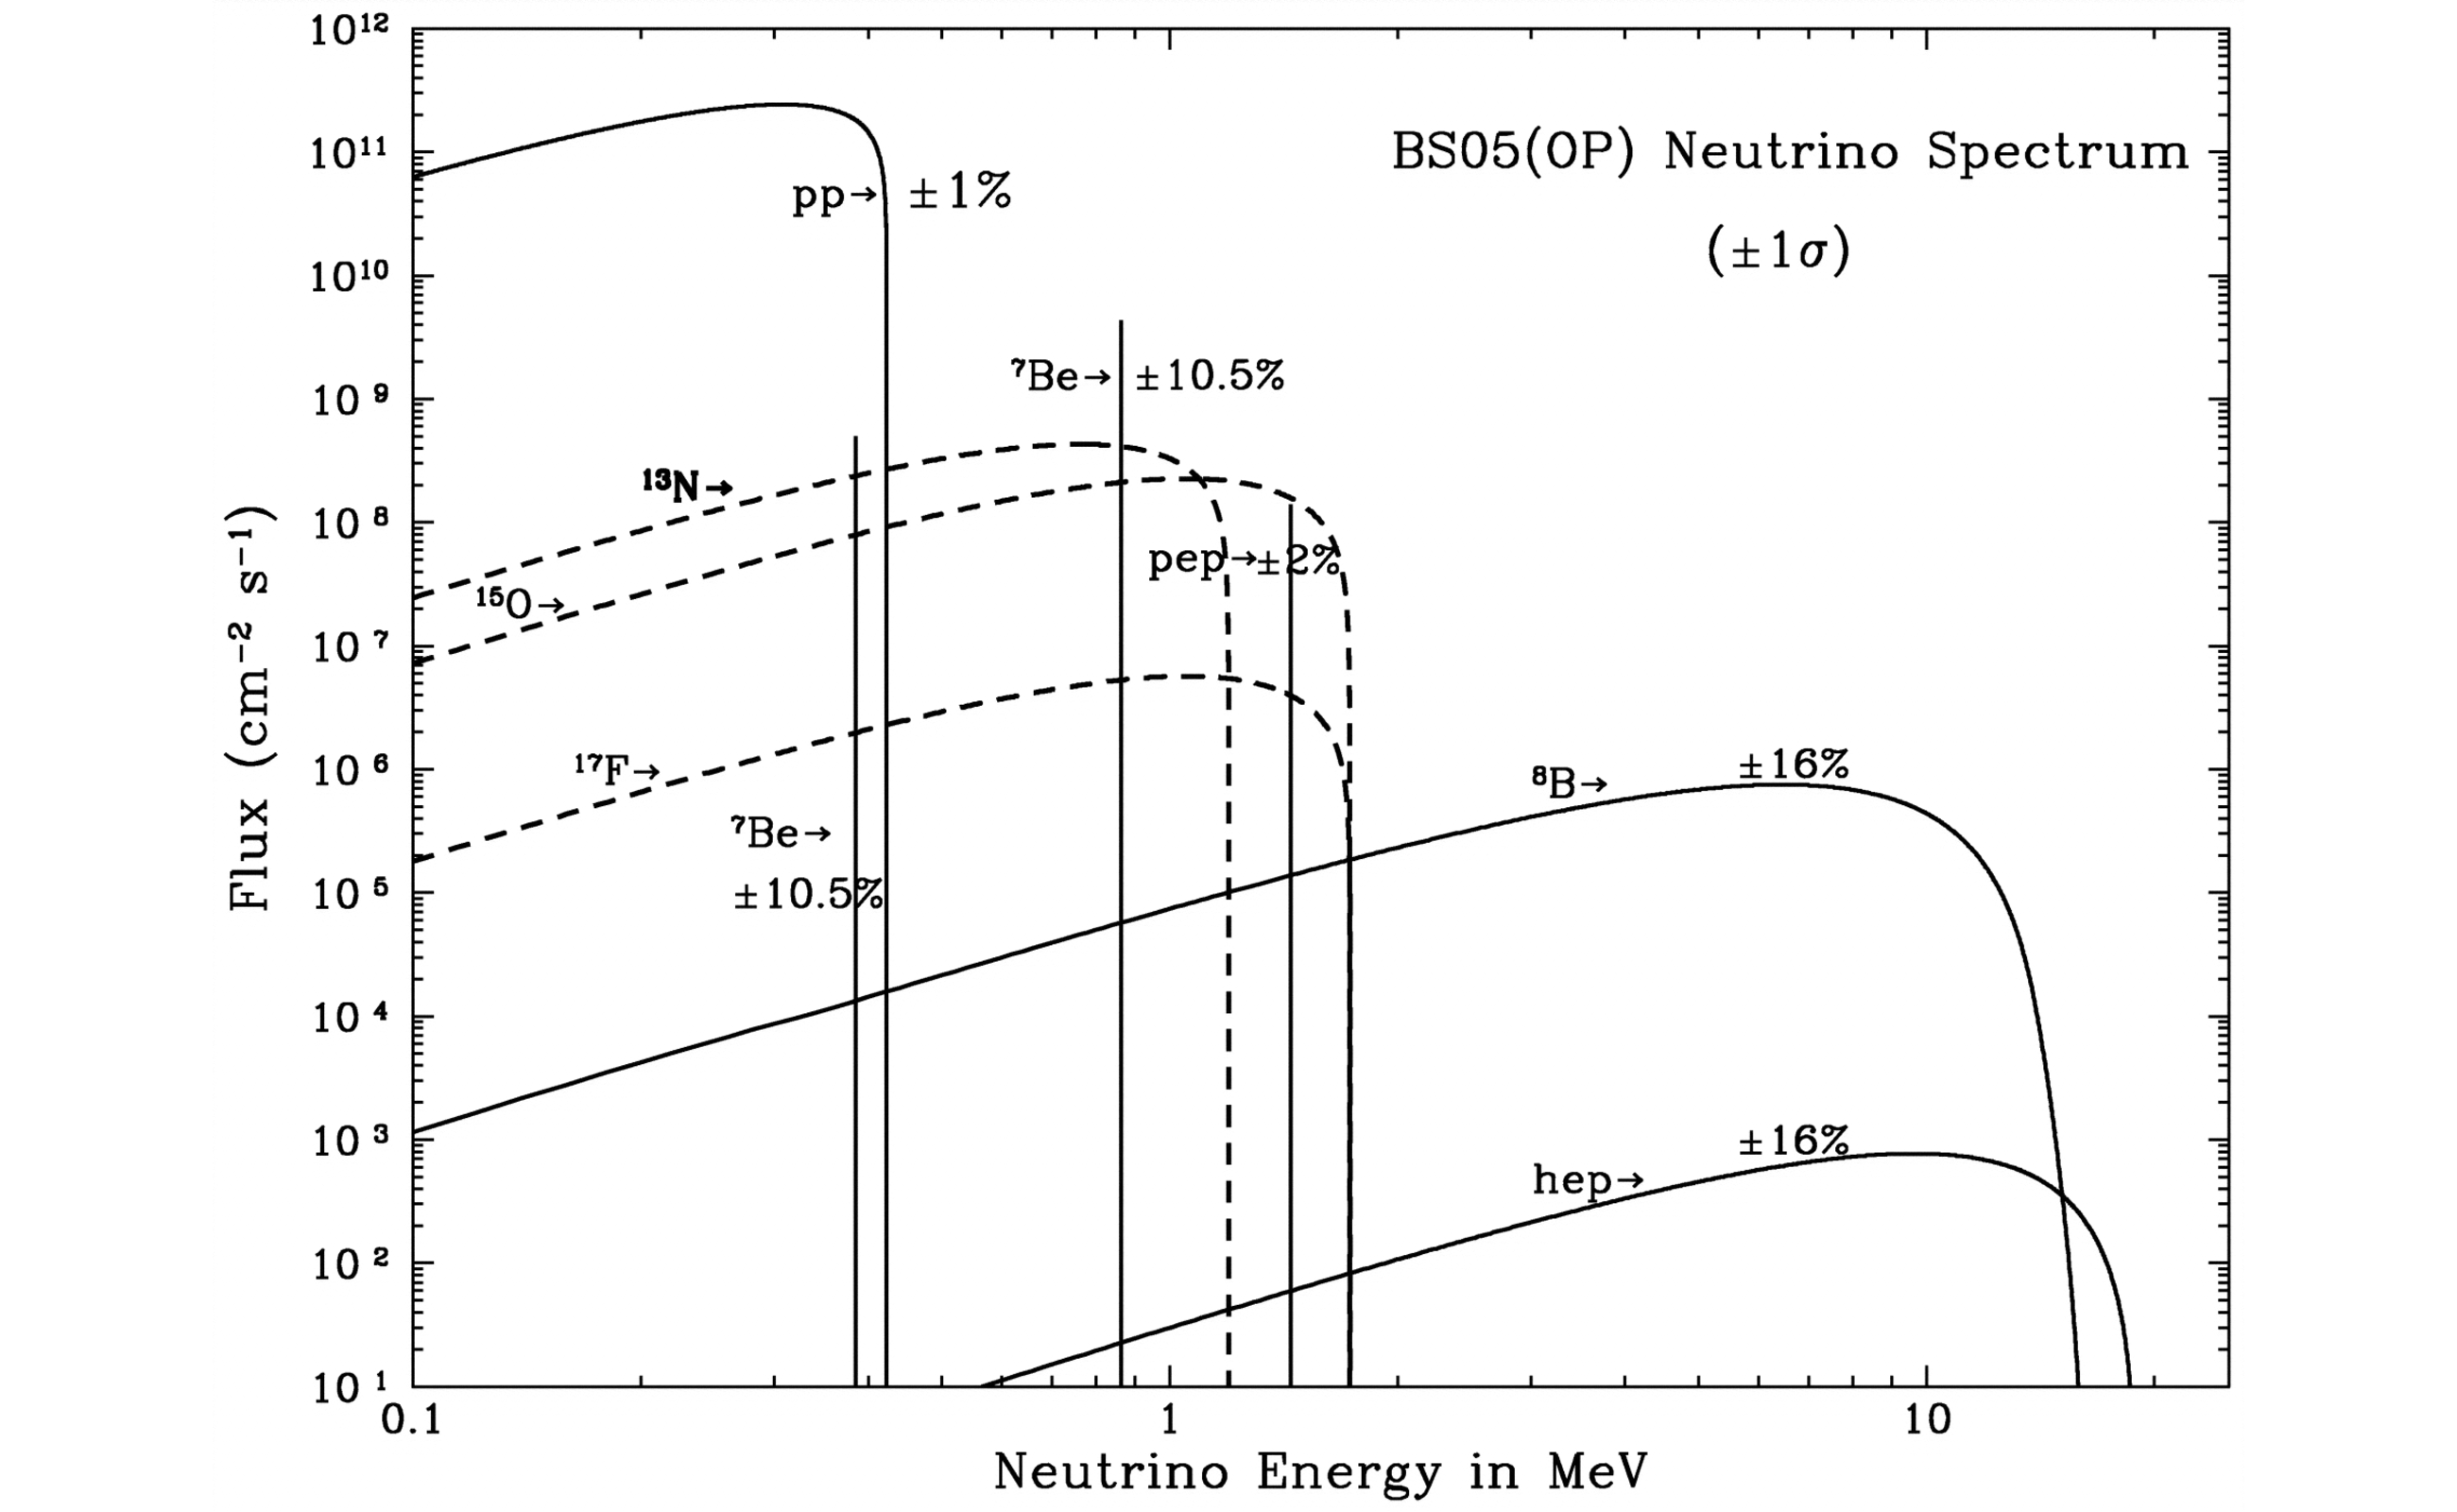
\includegraphics[width=0.8\textwidth]{img/bahcallserenelli.pdf}
    \caption{Solar neutrino energy spectrum for the solar model BS05(OP). The uncertainties are taken from Table 8 of \cite{2005ApJ...621L..85B}.}
    \label{fgr:bahcallserenelli}
\end{figure}
\par The sharper amongst my readers will have surely noticed that there are some elements which are simultaneously involved in destruction and production processes (e.g., $\element{D}{2}{1}$ or $\element{He}{3}{2}$). These elements are usually called \emph{secondary elements}.
\par It should come as no surprise that the variation of the abundance of element $i$ will depend on all the creation and destruction reactions involving that element\footnote{The general equation is quite long and convoluted, and I see no point into copying it here. The interested reader can refer to \cite{2005essp.book.....S}, §3.17, equation 3.39.}. If you recall how we've defined the reactoin rate (\ref{eq:reactionrate}), we can then say that the variation over time of the abundance (or number of particles) of a certain species will be 
\begin{equation*}
    \dot{N}_{i} = r_{i}^{C}-r_{i}^{D}
\end{equation*}
\par Let us consider for example, the equilibrium equation for Deuterion
\begin{equation*}
    \dot{N}_{\text{D}} = \frac{N_{p}N_{p}}{2}\langle \sigma v \rangle_{pp}-N_{\text{D}}N_{p}\langle \sigma v \rangle_{\text{D}p}
\end{equation*}
Equilibrium will be thus reached when $\dot{N}_{\text{D}} = 0$, so when
\begin{equation*}
    \frac{N_{\text{D}}}{N_{p}} = \frac{\langle \sigma v \rangle_{pp}}{2\langle \sigma v \rangle_{\text{D}p}}
\end{equation*}
What do we learn from this? The equilibrium abundance is \emph{directly proportional} to the creation rate and \emph{inversely proportional} to the destruction rate.
\par It is evendent that if the abundance of $\element{D}{2}{1}$ is larger than its abundance at equilibrium, then the destruction process prevails over the production one, and the chemical abundance will tend to evolve quickly towards its equilibrium configuration.
\par Under the assumption that $N_{\text{D}} \gg N_{\text{D}, \text{eq}}$ we can determine a timescale for the process, since the destruction process will be dominating
\begin{equation}
    \der{N_{\text{D}}}{t} = -N_{\text{D}}N_{p}\langle \sigma v \rangle_{\text{D}p}
    \label{eq:deuterionequilibrium}
\end{equation}
whose solution is of the type $N_{\text{D}} = N_{\text{D},0}\exp(-t/\tau)$, with
\begin{equation}
    \tau = \frac{1}{N_{p}\langle \sigma v \rangle_{\text{D}p}}
    \label{eq:deuteriontimescale}
\end{equation}
\par For typical temperatures at which the p-p chain is fully efficient, the value of $\tau$ is of the order of $1\unit{s}$, meaning the equilibrium configuration is reached quite hastily.
\par From this we're learning also something else really important: With given initial conditions, the reaction chain can reach and (virtually) remain in equilibrium, but the reaction rate will be led by the slower reaction which (\ref{eq:deuteriontimescale}) tells us is that with the smaller cross section.
\par In the p-p chain, the reaction telling the time to the others is the very first one, which has, as we've seen, an abysmally small cross section
\begin{equation*}
    \sigma_{\text{pp}}\sim 10^{-23}\unit{b} \quad S(0)_{pp}\sim 4.1\cdot 10^{-22}\unit{keV}\unit{b}^{-1}
\end{equation*}
which, for example, we can compare to the very following reaction, the one involving deuterion, that has $S(0)_{\text{D}p}\sim 2.1\cdot 10^{-4}\unit{keV}\unit{b}^{-1}$.
\par So there are 18 orders of magnitude of difference.
\subsection{Hydrogen Burning: CN-NO}
The CN-NO (by)cycle is the combination of two independent cycles: The CN cycle and the NO cycle. The presence of some isotopes of Carbon, Nitrogen and Oxygen are necessary for either cycle to begin. Being both produced and destroyed during these cycles, those elements act as catalysts. The reaction networks involved are the following:
\begin{align*}
    & \text{\textbf{CN cycle}}\\
    & \element{C}{12}{6}+\element{p}{1}{1}\to \element{N}{13}{7}+\gamma\\
    & \element{N}{13}{7}\to \element{C}{13}{6}+e^{+}+\nu_{e}\\
    & \element{C}{13}{6}+\element{p}{1}{1}\to \element{N}{14}{7}+\gamma\\
    & \element{N}{14}{7}+\element{p}{1}{1}\to \element{O}{15}{8}+\gamma\\
    & \element{O}{15}{8}\to \element{N}{15}{7}+e^{+}+\nu_{e}\\
    & \element{N}{15}{7}+\element{p}{1}{1}\to \element{O}{16}{8}^{*}\to \element{C}{12}{6}+\element{He}{4}{2} \;\; (\Gamma \sim 99\%)\\
    &\quad \quad \quad \quad\to \element{O}{16}{8}+\gamma\quad \quad \quad \quad \quad\,(\Gamma \sim 1\%)
\end{align*}
This branch of the cycle has to follow the timescale of $\element{N}{14}{7}+\element{p}{1}{1}\to \element{O}{15}{8}+\gamma$, which has the smaller cross section, folloed by the first reaction of the cycle.